\section{Introduction to statistics}

Here's how this tutoring thing is gonna go. First we will cover basic probability and stat theory, then we will cover each statistical test that your course pdf listed. For each test, we will do a short maths intro then move on to maths practice problems then practice in Jamovi. Every time we learn a new concept, I will have a new document on that topic written up. The list of tests and the order in which we will cover them is
\begin{enumerate}
    \item tbd...
\end{enumerate}
Things I can change. Amount of time we meet each week (length of each session, number of sessions per week), topics covered (we might be spending too much time on a topic that is important but that you already understand among other reasons), the amount of intro maths explanation for each, amount of maths questions, amount of Jamovi practice. Regarding the readings, you can ask me to change the length of the reading, the amount of maths, the tone used (too conversational? too serious?), or the type of content (maybe more examples and less abstract with the concepts?). Obviously feel free to ask me to change stuff outside of this list since I may not have thought of everything and I will do my best.

Based on what I've seen from the textbook and class notes, the goal of the stats courses you are going through seem to be to give you the bare minimum amount of theoretical knowledge to answer questions about data that you might encounter as a psychologist using the statistical tests they want you to be proficient with. I will try and follow this idea but clearly what I consider the acceptable amount of theoretical knowledge to be using statistical concepts in real life is different from what the people who designed your course think. I also think that more than just statistical tests should be used to answer questions about data but I don't know what a psychologist might need or if you will be taught that in the future so I will let that go for now. If you think I am ever focusing too much on the maths and not the problems solving, tell me and I will fix that.

So before we get into all the fancy mathy bits about understanding stats and all that, I hope that this intro will show you the importance of being very precise about what each concept in maths or stats means and how being precise can help you in both your exams and thinking about stats in general.

\subsection{The logic behind mathematics}

So your textbook argues that teaching statistics without maths is beneficial to students because the authors believe it should be the case that "understanding a very concrete concept such as the arithmetical mean would be a good deal easier than understanding a rather vague psychological concept such as 'an attitude" (p.1). This is interesting for two reasons. The first is that it suggests that the arithmetic mean is not only more concrete than 'an attitude' but is also simpler than all the forms that 'an attitude' can take. The second is that the authors seem to be under the misunderstanding that a more "concrete" concept should be easier to understand than a "vague" one.

Let's look at the first point and ask if the arithmetic mean is a less complex idea than whatever 'an attitude' is in psychology. The arithmetic mean is a popular idea that everyone with any level of education in probability or statistics will be somewhat familiar with.

So now we turn to our second point. An acceptable verbal definition of the arithmetic mean in a conversational context when applied to a psychological experiment may be "the attitude that a normal person takes". In an psychological experiment, it is almost certainly true that if we take the arithmetic mean of some data set that we want to try and find some number that represents the behaviour of a "normal" or "middling" person. However, if your data has two peaks like the figure below, would it be correct to say that the arithmetic mean is a good representation of "normal", "average", "middling", or some other synonym of a typical subject? \\

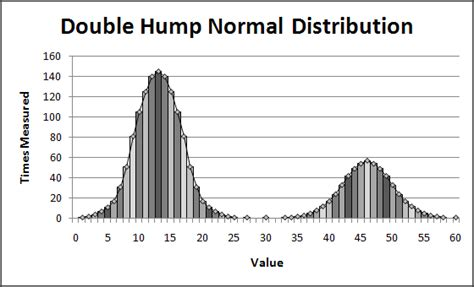
\includegraphics[scale=.7]{images/double_hump.jpg} \\

If we just told everyone that the arithmetic mean meant that it is the value that occurs the most, it would be confused as the mode, but if we told everyone it is a value that is probably somewhere in the middle, it would be confused as the median.

However, I will agree that in almost all stats courses, the interpretation of the maths is underemphasised and that students would have a much easier time learning what the maths means in words than just working with fancy symbols. My approach will be different from the book in that I will show you all these complicated looking mathematics, treat these fancy symbols as something like another language and translate them back into English, and hopefully when you think of stats in the future you can think about how the logic connects instead of just "well I've passed the t- or z-test, whatever that means, so my findings are correct". I hope that all my explanations will lay out clearly, both what the mathematical statements that we will learn mean, and also just as importantly (as we have seen the previous paragraphs), what they do not mean.

\hyperlink{https://en.wikipedia.org/wiki/Analysis_of_variance}{imp topic (anova)}